\chapter{Continuous time finance}\lesson{9}{27/03/2020}
\section{Stochastic integrals}% pag. 300 in poi Hull
The starting point for finance in continuous time is a probability space $$(\Omega,\mathcal{F},\{\mathcal{F}_t\}_{t\ge0},\mathbb{P}),$$ where $\{\mathcal{F}_t\}_{t\ge0}$ is an increasing family of complete $\sigma$-algebras. Here, in order to avoid measurability problems, we assume also that $\{\mathcal{F}_t\}_{t\ge0}$ has right continuity:
\begin{equation*}
    \bigcap_{\epsilon>0}\mathcal{F}_{t+\epsilon}=\mathcal{F}_{t^+} = \mathcal{F}_t
\end{equation*}
This means that the information available immediately after $t$ coincides with the one at time $t$, so there can be shocks only in the left side of the limit, which can be discontinuous. This is a quite heavy assumption, because it involves the future, but it is compulsory. In this probability space we define the underlying stochastic process $X_t$ and we assume measurability with respect to the probability infrastructure and regularity in terms of the trajectory. In particular, we assume that $X_t$ is a \emph{RCLL} function, also called \emph{càdlàg}, i.e. a function defined on the real numbers (or a subset of them) that is right-continuous everywhere and has left limits everywhere.
\begin{figure}[htp]
    \centering
    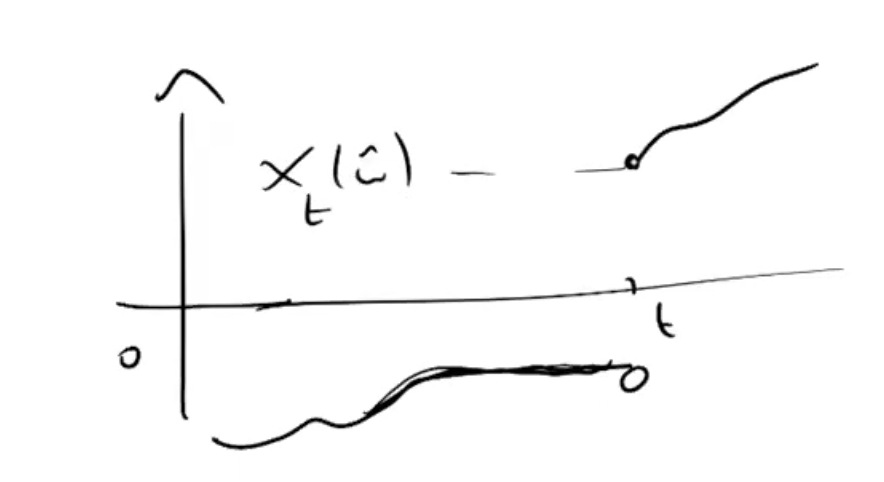
\includegraphics[scale=0.3]{fig/tmp/fig9.png}
    \caption{Càdlàg.}
    \label{fig:càdlàg}
\end{figure}
\newline Processes like this define a \emph{Brownian motion} $W_t$, i.e. a gaussian process with distribution at fixed time $\hat{t}$ $W_{\hat{t}}\sim\mathcal{N}(0,\hat{t})\sim\sqrt{\hat{t}}\mathcal{N}(0,1)$. Then we can define the stochastic integral
\begin{equation*}
    \int_0^t H_s\,``\dd W_s"
\end{equation*}
where $H\in\mathcal{H}$, being $\mathcal{H}$ the class of adapted processes such that $\mathbb{E}[\int_0^t H^2_s\,\dd s]<\infty$.
% completare questa parte mettendo qualcosa degli appunti di models, anche riguardo al fatto che il Brownian motion non è differenziabile ma si può definire una misura e calcolare formalmente un integrale bla bla bla
Since the Brownian motion is not differentiable it is not possible to define a differential. However, if we are able to define the integral with respect to the Brownian motion then we can define the differential operator as the derivative of the integral:
\begin{equation*}
    \dd\left(\int^t_0 H_s \dd W_s\right) \to H_t``\dd W_t"
\end{equation*}
\begin{example}{}{}{}
    Consider a process given by the deterministic integral
    \begin{equation*}
        X_t = \int^t_0 W_s\dd s
    \end{equation*}
    where $W_s$ is a Brownian motion. We want to show that $X_t$ behaves like a gaussian random variable $\mathcal{N}(\mu,\sigma)$ where $\mu, \sigma$ have to be determined. To solve the integral we can use \emph{Itô's Lemma}:
    \begin{equation*}
        \dd(tW_t) = W\dd t + t\,\dd W_t + \underbrace{\dd\langle\cdot,W_{\cdot}\rangle_t}_{\sim 0}
    \end{equation*}
    where $t$ is deterministic and the last term -- the quadratic covariance -- can be neglected because it leads to higher order terms in $\dd t$ (recall that $\dd t\dd W = \dd t\sqrt{\dd t}$). Integrating by parts we get:
    \begin{equation*}
        tW_t = \int^t_0 W_s\,\dd s + \int^t_0 s\,\dd W_s
    \end{equation*}
    So we can say that the integral
    \begin{equation*}
        \int^t_0 W_s\dd s = tW_t - \int^t_0 s\,\dd W_s
    \end{equation*}
    is Guassian, being the sum of two gaussian terms. \\
    Alternatively, recall that it is always possible to consider the Brownian motion as the integral of its differential, in fact we can define the integral operator to be compatible with the differential one:
    \begin{equation*}
        W_t = \int^t_0 \dd W_s = W_t - W_0
    \end{equation*}
    So, we can write:
    \begin{align*}
        \int^t_0 W_s\dd s &= \int^t_0\left(\int^s_0 \dd W_u\right)\,\dd s \overset{(a)}{=} \int^t_0\left(\int^t_u \dd s\right)\dd W_u \\
        &=
        \int^t_0(t-u)\,\dd W_u = tW_t - \int^t_0\dd W_u
    \end{align*}
    where in (a) we used the Stochastic Fubini Theorem to change the order of integration.\\
    Now we look for $\mu$ and $\sigma$. We have that
    \begin{equation*}
        \mathbb{E}[X_t] = \mathbb{E}\left[\int^t_0 W_s\,\dd s \right] \overset{(a)}{=} \int^t_0 \mathbb{E}[W_s]\dd s \overset{(b)}{=} 0
    \end{equation*}
    where in (a) we moved the expectation value inside the integral (we can do it because it is a deterministic integral) and in (b) we used the fact that by definition $\mathbb{E}[W_s] = 0$. Then:
    \begin{align*}
        \Var(X_t) &= \mathbb{E}\left[\left(\int^t_0 W_s\,\dd s \right)^2\right] = \mathbb{E}\left[\int^t_0\int^t_0 W_sW_u\,\dd s\,\dd u \right]\\
        &=
        \int^t_0\int^t_0 \mathbb{E}[W_sW_u]\dd s\,\dd u =
        \int^t_0\int^t_0 \Cov(W_s,W_u)\dd s\,\dd u
        \intertext{The increments of the Brownian motion are independent but the brownian motion itself is a strongly autocorrelated process, with covariance $\Cov(W_t,W_u)=\min\{s,u\}$. So we can write:}
        &=
        \int^t_0\left(\int^u_0 s\,\dd s+\int^t_u u\,\dd s\right)\dd u = \int^t_0\left(\dfrac{u^2}{2}+u(t-u)\right)\dd u \\
        &=
        \dfrac{t^3}{6}+\dfrac{t^3}{2}-\dfrac{t^3}{3} =  \dfrac{t^3}{3}
    \end{align*}
    So $X_t\sim\mathcal{N}(0,\nicefrac{t^3}{3})$.\\
    \textbf{Warning!} In this example we are able to do the computations -- in particular we can switch expected value and integration -- because we are dealing with deterministic integrals. If we have a stochastic integral, e.g. $\int^t_0H_s\dd W_s$, we cannot move the expected value inside the integral because we get something which is random:
    \begin{equation*}
        \underbrace{\mathbb{E}\left[\int^t_0H_s\dd W_s\right]}_{deterministic} \ne \underbrace{\int^t_0\mathbb{E}[H_s]\dd W_s}_{stochastic}.
    \end{equation*}
\end{example}
\noindent An important property is that if $H_s\in\mathcal{H}$, then the stochastic process $$\left(\int^t_0H_s\dd W_s\right)_{t\ge0}$$
is a martingale:
\begin{equation}
    \mathbb{E}\left[\int^t_0H_s\dd W_s\right] = \int^0_0H_s\dd W_s = 0.
\end{equation}
Luckily, $\mathcal{H}$ is a very rich class which contains also Brownian motions. In fact:
\begin{align*}
    \mathbb{E}\left[\int^t_0W_s^2\dd s\right] &= \int^t_0\mathbb{E}[W_s^2]\,\dd s = \int^t_0\Var(W_s)\,\dd s = \int^t_0s\,\dd s = \dfrac{t^2}{2} < \infty.
\end{align*}
We can extend the notion of stochastic integral even when $H_s\notin\mathcal{H}$, requiring a weaker condition, i.e.
\begin{equation*}
    H_s \in \Tilde{\mathcal{H}} = \bigg\{H\mbox{ adapted }: \mathbb{P}\left(\int_0^t H^2_s\,\dd s <\infty\right)=1\bigg\},
\end{equation*}
but in this case $X_t$ is a \emph{local martingale}, meaning that it is a martingale only for a specific set of stopping times. This means, in principle, that $\mathbb{E}[X_t]\ne0$.\\
Now, consider a Geometric Brownian Motion (GBM)
\begin{equation}
    \begin{cases}
    \dd X_t = \alpha X_t\, \dd t + \sigma X_t\, \dd W_t\\
    X_0 = x_0,
    \end{cases}
\end{equation}
which also can be written as
\begin{equation}
    X_t - x_0 = \alpha\int^t_0 X_s\, \dd s + \sigma\int^t_0 X_s \,\dd W_s.
\end{equation}
Since we are dealing with stochastic integrals, trivial integration is not possible and we have to find an other way to compute them. \\
First, let's consider the case in which $\sigma=0$. We get a linear deterministic equation:
\begin{equation}
    \dd X_t = \alpha X_t\, \dd t
\end{equation}
which can be written as
\begin{equation}
    \Dot{X}_t = \dv{X_t}{t} = \alpha X_t
\end{equation}
and has solution
\begin{equation}\label{detsol}
    X_t = x_0e^{\alpha t}.
\end{equation}
If $\sigma\ne0$ it is as we introduce a white noise which disturbs the evolution of the deterministic solution. The naive approach is to write the solution as
\begin{equation}
    X_t = ``x_0e^{\alpha t + \sigma W_t}"
\end{equation}
This is not correct, becayse it means that we are considering the exponential in a deterministic way, which is not the case. We have to use Itô's Formula.
\begin{theorem}[Itô's Formula]
    Assume that the process $X$ has a stochastic differential given by
    \begin{equation}
    \begin{cases}
        \dd X_t = K_t\, \dd t + H_t\, \dd W_t\\
        X_0 = x_0
    \end{cases}
    \end{equation}
    where $\alpha$ and $\sigma$ are adapted processes ($\alpha,\sigma\in\Tilde{\mathcal{H}}$), and let $f$ be a $C^{1,2}$ function. Define the process $Z(t) = f(t,X(t))$. Then $Z$ has a stochastic differential given by
    \begin{equation}\label{ito}
        \dd f=\left({\frac{\partial f}{\partial t}}+K_{t}{\frac {\partial f}{\partial x}}+{\frac{H_{t}^{2}}{2}}{\frac{\partial ^{2}f}{\partial x^{2}}}\right)\dd t+H_{t}{\frac{\partial f}{\partial x}}\,\dd W_{t}.
    \end{equation}
\end{theorem}
In our case, we take $f$ as the function which simplifies the deterministic part, which is an exponential. So, we take:
\begin{equation}
    f(t,X_t) = \ln X_t.
\end{equation}
According to \eqref{ito}, the differential is:
\begin{align}
    \notag \dd\ln{X_t} &= \dfrac{1}{X_t}\,\dd X_t + \dfrac{1}{2}\left(-\dfrac{1}{X_t^2}\right)\,\dd \expval{X_t}_t \\
    &=
    \notag \alpha\,\dd t + \sigma\,\dd W_t - \dfrac{1}{2X_t^2}(\sigma^2X_t^2\,\dd t)\\
    &=
    \left(\alpha-\dfrac{1}{2}\sigma^2\right)\,\dd t + \sigma\,\dd W_t
\end{align}
and integrating both sides we get:
\begin{equation}
    \ln X_t - \ln X_0 = \left(\alpha-\dfrac{1}{2}\sigma^2\right)t + \sigma(W_t-W_0) = \left(\alpha-\dfrac{1}{2}\sigma^2\right)t + \sigma W_t
\end{equation}
By taking the exponential of both sides we get:
\begin{equation}\label{stocsol}
    X_t = x_0e^{\left(\alpha-\frac{1}{2}\sigma^2\right)t + \sigma W_t}
\end{equation}
Notice that this solution is log-normal:
\begin{equation*}
    X_t \sim e^{\mathcal{N}\left(\ln x_0 + \left(\alpha-\frac{1}{2}\sigma^2\right)t, \sigma^2 t\right)}
\end{equation*}
and that it fluctuates around the corresponding deterministic solution \eqref{detsol}. We can demonstrate that averaging \eqref{stocsol} we get exactly \eqref{detsol}, in fact -- according to the moment generating function formula ${M(t)=\mathbb{E}[e^{tX}]=e^{\mu t}e^{{\frac {1}{2}}\sigma^{2}t^{2}}}$ -- the expected value of $e^{-\frac{1}{2}\sigma^2 t + \sigma W_t}$ is:
\begin{equation*}
    \mathbb{E}\left[e^{-\frac{1}{2}\sigma^2 t + \sigma W_t}\right] = \mathbb{E}\left[
    e^{\mathcal{N}\left(-\frac{1}{2}\sigma^2 t, \sigma^2 t\right)}\right] = e^{-\frac{1}{2}\sigma^2 t + \frac{1}{2}\sigma^2 t} = 1
\end{equation*}
Alternatively, one may recognize that $e^{-\frac{1}{2}\sigma^2 t + \sigma W_t}$ is a famous exponential martingale $Y_t$, and so $\mathbb{E}[Y_t]=Y_0=e^0 = 1$.

\subsection{Black \& Scholes market} % pag. 321 Hull
In the early 1970s, Fischer Black, Myron Scholes and Robert Merton achieved a major breakthrough in the pricing of European stock options. This was the development of what has become known as the Black–Scholes–Merton (Black \& Scholes) model.
This model describes the asset price $S_t$ in terms of the infinitesimal return $\frac{\dd S_t}{S_t}$, assuming that percentage changes in the stock price in a very short period of time are normally distributed. If we define a drift $\mu$ as the \emph{expected return of a stock per year}  and $\sigma$ as the \emph{volatility of the stock price per year} (a measure of our uncertainty about the returns provided by the stock), we have that
\begin{equation}\label{bs}
    \frac{\dd S_t}{S_t} = \mu \dd t + \sigma\dd W_t
\end{equation}
where $\dd W_t$ represents the noise given by this variability. The mean and standard deviation of the return in time $\dd t$ are approximately $\mu\dd t$ and $\sigma\sqrt{\dd t}$, so that
\begin{equation}
    \frac{\dd S_t}{S_t} \sim \mathcal{N}(\mu\dd t, \sigma^2\dd t)
\end{equation}
Recalling what we saw in the previous section, this implies that the return $Y_t = \ln S_t$ is normally distributed:
\begin{equation}
    \ln S_t \sim\mathcal{N}\left(\ln S_0+\left(\mu-\dfrac{\sigma^2}{2}\right)t,\sigma^2 t\right)
\end{equation}
and so $S_t$ is log-normal distributed.
\begin{figure}[htp]
    \centering
    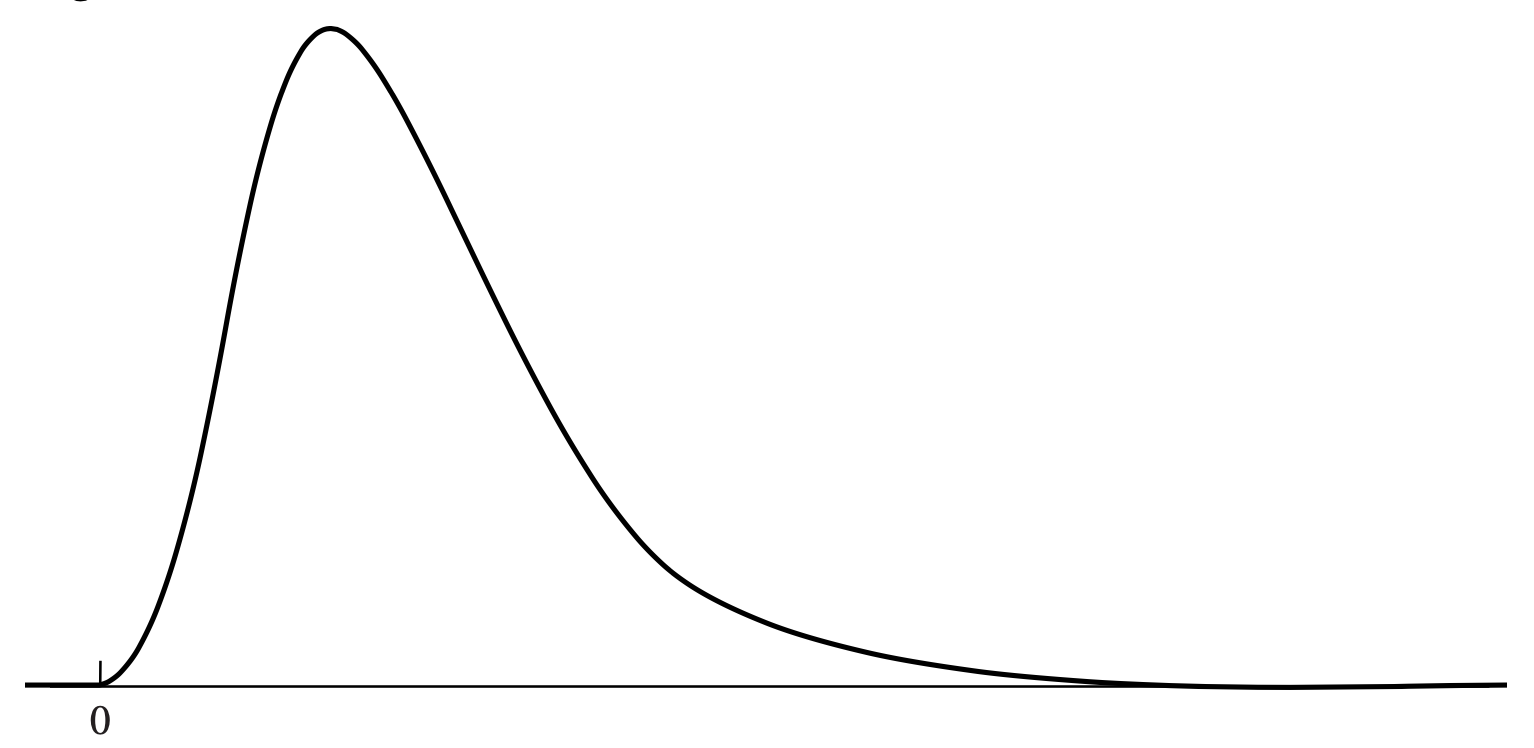
\includegraphics[scale=0.2]{fig/log_norm_distr.png}
    \caption{Log-normal distribution}
    \label{fig:lognorm}
\end{figure}
\newline While it is possible to estimate the historical volatility of the market, it is not possible to estimate the historical drift because it is not observable and also not stable. In fact, according to the particular time window we are considering, $\mu$ can assume different values.
\begin{figure}[htp]
    \centering
    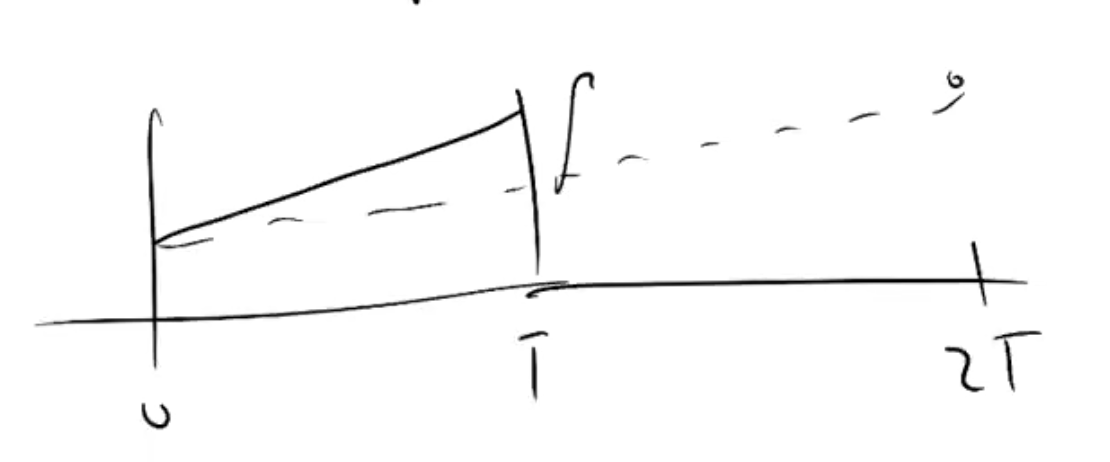
\includegraphics[scale=0.3]{fig/tmp/fig11.png}
    \caption{Different values of $\mu$.}
    \label{fig:mu}
\end{figure}
\newline In conclusion, we cannot jointly estimate $\mu$ and $\sigma$ from only one time series and we would like to get results which are independent of the drift (which plays the same role as the subjective probability in the static binomial model).

\subsection{The Girsanov Theorem} % pag. 162 Bjork
We want to find a way to switch from the subjective probability measure $\mathbb{P}$ to $\mathbb{Q}$ in continuous time. The tool that allows us to do that is the Girsanov Theorem.\\
Consider a Brownian motion $W_t^{\mathbb{P}}$ under the probability measure $(\Omega, \mathcal{F}, \mathbb{P})$ and a \emph{finite variation process} $\int^t_0 H_s\,\dd s$ (its differential has not a diffusion part). Then
\begin{equation}
    W_t^{\mathbb{Q}} \coloneqq W_t^{\mathbb{P}} - \int^t_0 H_s\,\dd s
\end{equation}
is not a Brownian motion under the measure $\mathbb{P}$, because it is not a martingale. However, it is a Brownian motion under the measure $\mathbb{Q}$, where
\begin{equation}\label{RN}
    \eval{\dv{\mathbb{Q}}{\mathbb{P}}}_t = \exp\left(\int^t_0 H_s\,\dd W_s^{\mathbb{P}}-\dfrac{1}{2}\int^t_0 H_s^2\,\dd s\right) \coloneqq Z_t
\end{equation}
is a process that satisfies the stochastic differential equation (SDE)
\begin{equation}
    \dd Z_t = H_t Z_t\,\dd W_t^\mathbb{P}
\end{equation}
and can be written as a constant plus a stochastic integral, which at least is a local martingale:
\begin{equation}
    Z_t = Z_0 + \int_0^t H_s Z_s\,\dd W_s^{\mathbb{P}}
\end{equation}
Eq. \eqref{RN} is called \emph{Radon-Nikodym derivative}: the choice of notation and the name of the function reflects the fact that it is analogous to a derivative in calculus, in the sense that it describes the rate of change of density of one measure with respect to another\footnote{See \url{https://en.wikipedia.org/wiki/Radon\%E2\%80\%93Nikodym_theorem}}. \\
One possible issue is that in the change from $\mathbb{P}$ to $\mathbb{Q}$ there can be a loss of probability mass, ending up with a $\mathbb{Q}$ which is not normalized to 1. In order to avoid that, $\int_0^t H_s Z_s\,\dd W_s^{\mathbb{P}}$ must be a global martingale. This is the assumption of Girsanov Theorem.
\begin{theorem}[Girsanov Theorem]
    Consider a Brownian motion under a probability measure $\mathbb{P}$. Then, a candidate Brownian motion under a different probability measure $\mathbb{Q}$ is a true $\mathbb{Q}$-Brownian motion if the change of measure characterized by $Z_t$ is a true martingale.
\end{theorem}
One consequence of this theorem is that changing measure is equivalent to shift the Brownian motion by a finite variation process. If we want to move from a probability measure to another, the effect on the SDE involves the drift, not the volatility.\\
How can we check the true martingality condition on $Z_t$? We know that if $H_sZ_s\in\mathcal{H}$ then $\int H_sZ_s\,\dd W_s$ is a martingale, but we cannot use this information because it involves $Z_s$ itself, which is unknown. In order to do that we use the \emph{Novikov condition}.
\begin{lemma}[Novikov condition]
    If
    \begin{equation}
        \mathbb{E}\left[e^{\frac{1}{2}\int^t_0 H_s^2\,\dd s}\right]<\infty
    \end{equation}
    then $Z_t$ is a true martingale.
\end{lemma}
\textbf{Summary.} In conclusion, suppose that $X$ is a random variable and we want to compute
\begin{equation*}
    \mathbb{E}[X] = \int_{\Omega}X\,\dd\mathbb{P} = \int_{\Omega}X(\omega)\mathbb{P}(\dd\omega).
\end{equation*}
If we don't know the distribution of $X$ under the probability measure $\mathbb{P}$ but we know it under an other probability measure $\mathbb{Q}$, it is possible to switch from $\mathbb{P}$ to $\mathbb{Q}$ using the change of measure
\begin{equation*}
    \mathbb{E}^{\mathbb{P}}[X] = \int X\dv{\mathbb{P}}{\mathbb{Q}}\,\dd\mathbb{Q} = \mathbb{E}^{\mathbb{Q}}\left[X\dv{\mathbb{P}}{\mathbb{Q}}\right]
\end{equation*}
This holds for all $X$. In particular, if we take $X=1$ then
\begin{equation*}
    1 = \mathbb{E}^{\mathbb{P}}[1] = \mathbb{E}^{\mathbb{Q}}\left[\dv{\mathbb{P}}{\mathbb{Q}}\right]
\end{equation*}
So, in order to avoid loss of probability mass, $\dv{\mathbb{P}}{\mathbb{Q}}$ must be a true martingale.
